\paragraph{V2 - Python}
Die Python Version 2 wurde komplett überarbeitet und viel einfacher und übersichtlicher gestaltet. Das Konzept der mehreren Auslagerungsplätze wurde verworfen und es wurde nur ein Auslagerungsplatz implementiert.

Zudem wurde die Architektur komplett überarbeitet. V2 ist basierend auf einer \Gls{statemachine}, die verschiedenen States sind in Abbildung \ref{fig:tower_controller_v1_state_machine} zu sehen.

\begin{figure}
  \centering
  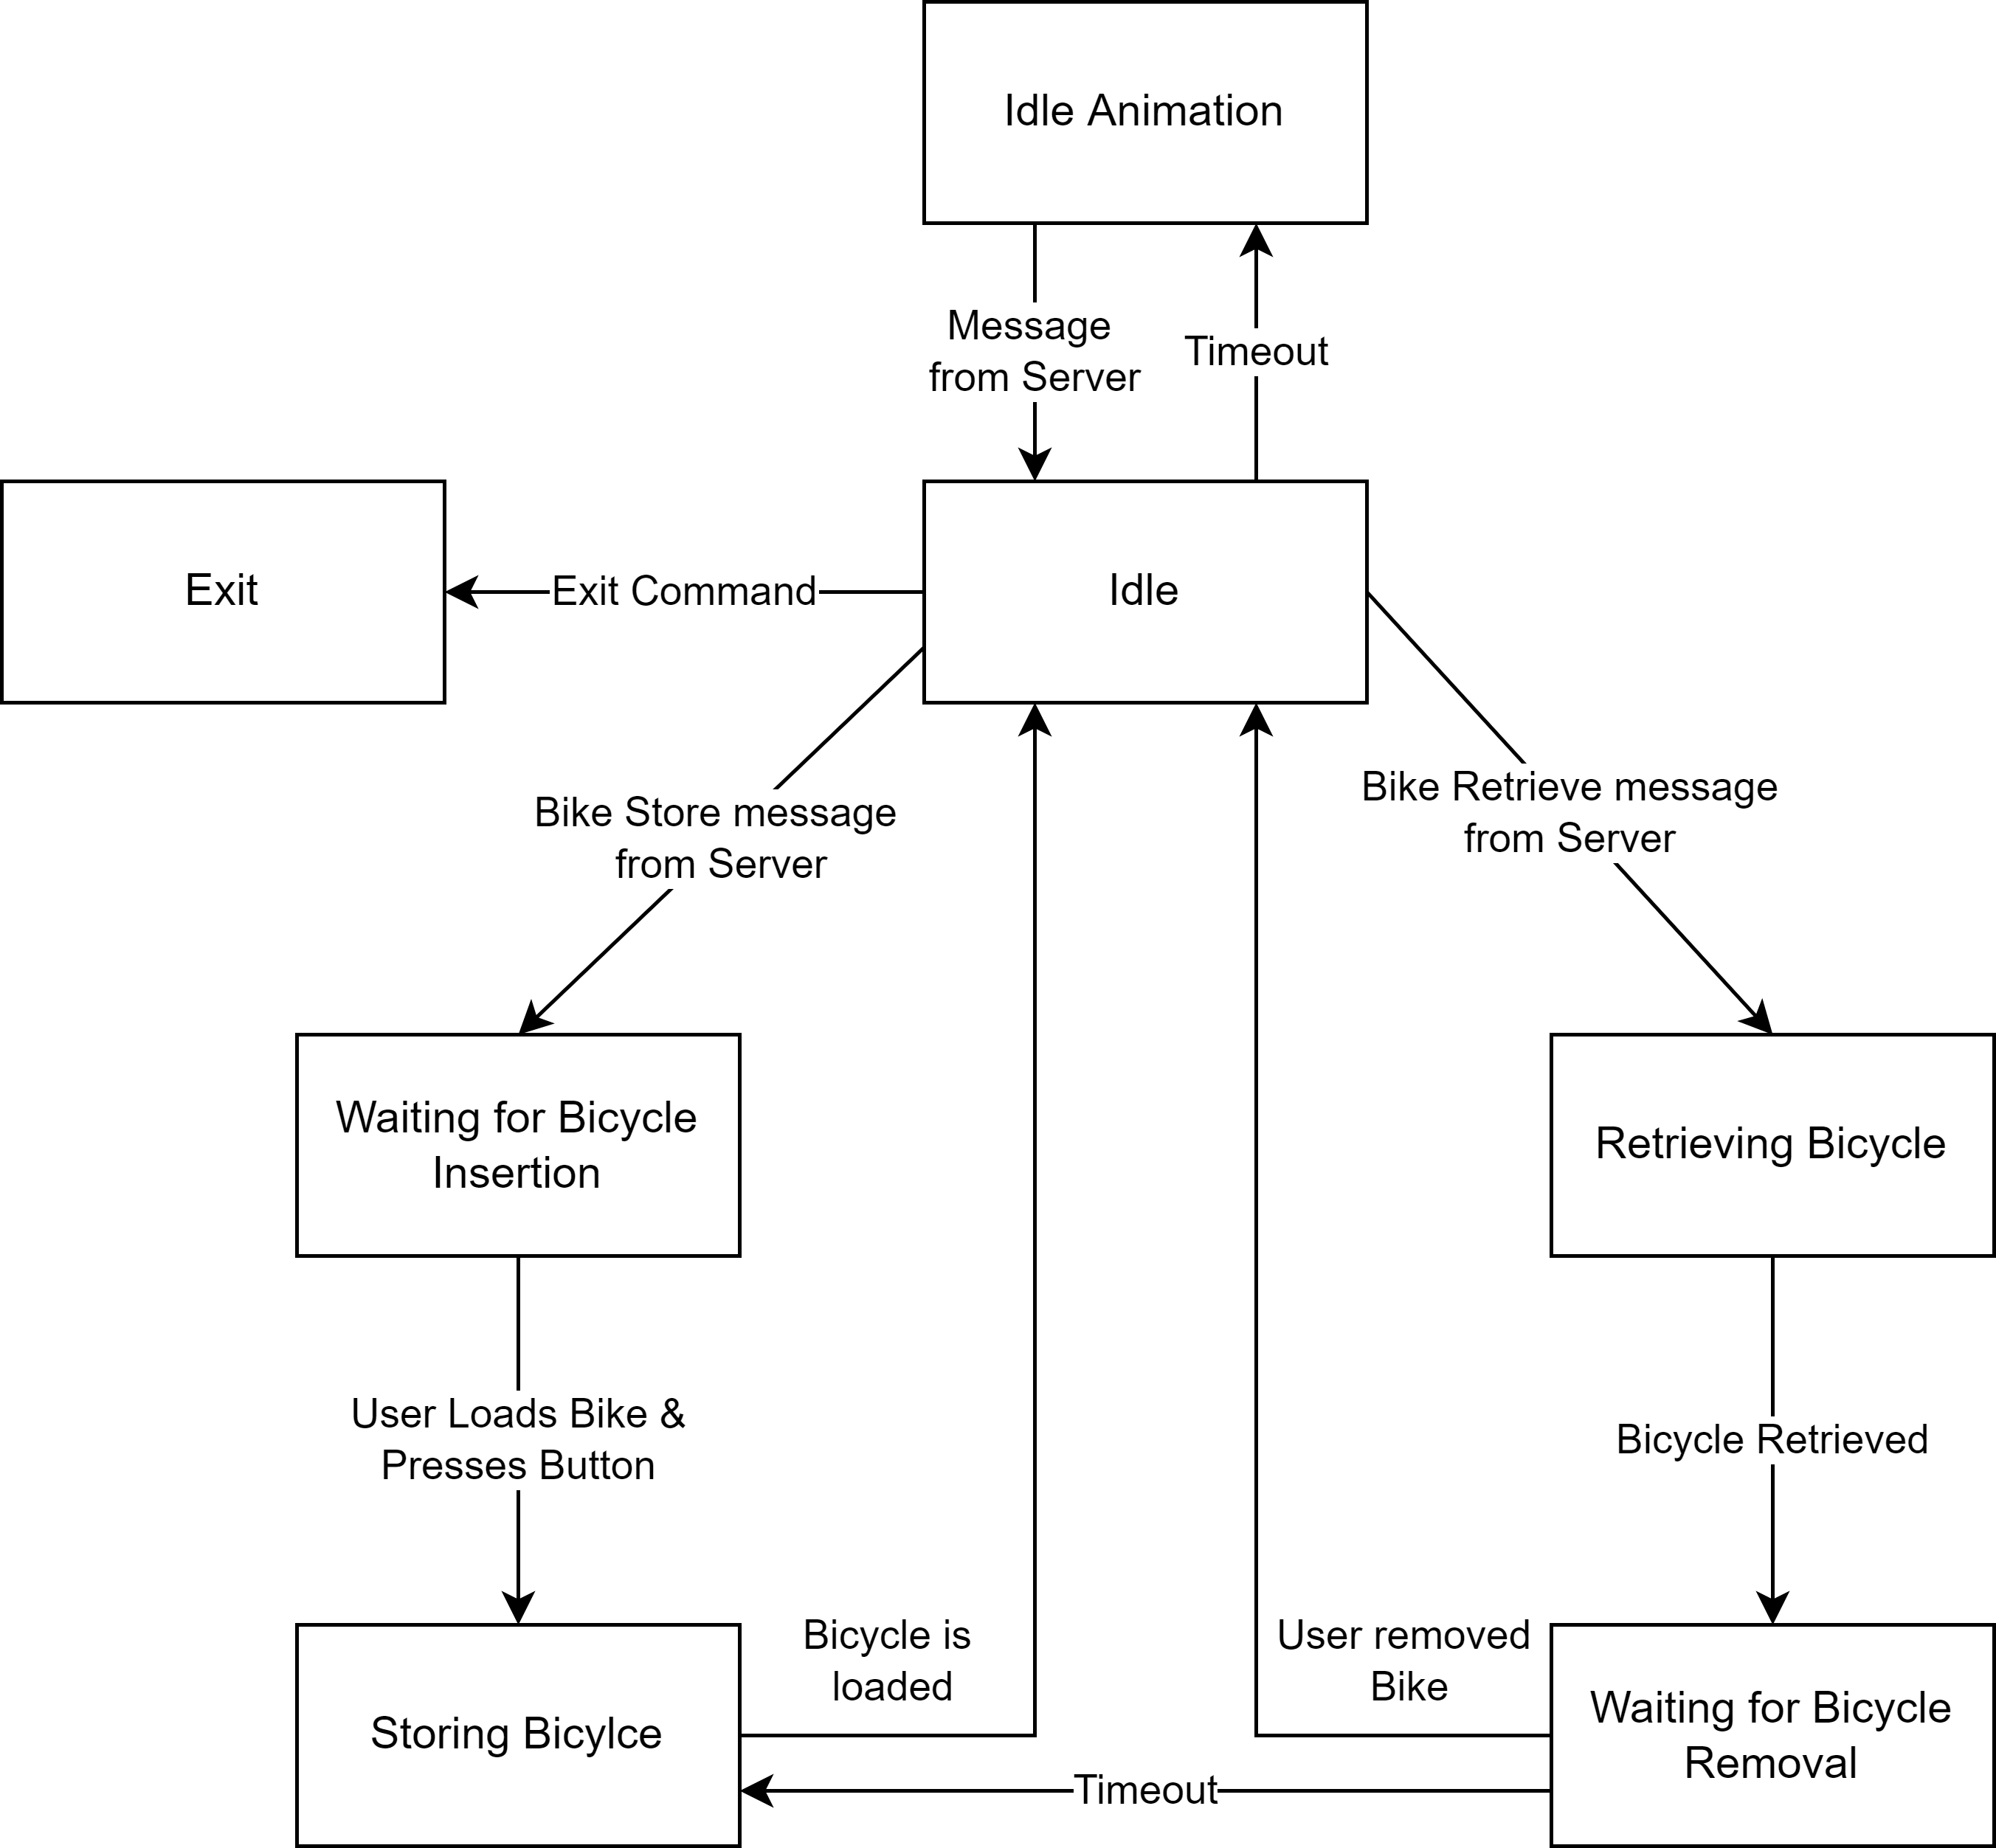
\includegraphics[width=0.8\textwidth]{images/tower_controller_v2_state_machine.png}
  \caption{State Machine des Tower Controller V2}
  \label{fig:tower_controller_v1_state_machine}
\end{figure}

States:
\begin{itemize}
  \item \textbf{Idle} - Der Turm ist im Idle State, wenn er nicht gerade eine Aktion ausführt. In diesem Zustand werden auf \Glspl{event} gewartet. Wenn ein \Gls{event} eintritt, wird der Zustand entsprechend angepasst.
  \item \textbf{Waiting for Bicycle Insertion} - Ein Nutzer hat den Einlagerungsprozess eines Fahrrads gestartet, der Turm wartet nun auf das Einlegen des Fahrrads in die Radbox und die Einlagerungsbestätigung (Drücken des Buttons) des Nutzers.
  \item \textbf{Storing Bicycle} - Das Fahrrad wurde in die Radbox eingelagert und der Nutzer hat die Einlagerungsbestätigung erteilt. Der Turm wartet nun auf das Schließen der Radbox und das Abschließen des Einlagerungsprozesses. Anschließend wird der Zustand wieder auf Idle gesetzt.
  \item \textbf{Retrieving Bicycle} - Ein Nutzer hat den Auslagerungsprozess eines Fahrrads gestartet, der Turm wartet nun auf das Abschließen des Auslagerungsprozesses und das Öffnen der Radbox.
  \item \textbf{Waiting for Bicycle Removal} - Der Turm wartet auf das Entfernen des Fahrrads aus der Radbox und die Auslagerungsbestätigung des Nutzers. Anschließend wird der Zustand wieder auf Idle gesetzt. Falls der Nutzer die Auslagerungsbestätigung innerhalb eines gewissen Zeitraums nicht erteilt, wird der Zustand wieder auf Storing Bicycle gesetzt und das Fahrrad wird eingelagert.
  \item \textbf{Idle Animation} - Falls der Turm für eine gewisse Zeit im Idle Zustand ist, wird eine Animation ausgeführt. Diese Animation soll den Turm visuell ansprechender machen.
  \item \textbf{Exit} - Der Turm Controller wird beendet.
\end{itemize}

Änhlich wie V1 hatte V2 auch eine \ac{GUI}, die den aktuellen Zustand des Turms darstellt. Diese wurde einfach von V1 übernommen und angepasst.

Die V2 Variante funktionierte gut und hätte womöglich auch Architekturell funktioniert, jedoch gab es Probleme mit Python selbst. Die Probleme stammten von zyklischen Importen und erlaubten es nicht die Entwicklung weiterzuführen. Womöglich hätte das Problem gelöst werden können indem auf Type Hints verzichtet worden wäre, jedoch hätte dies die Developer Experience und Lesbarkeit des Codes stark beeinträchtigt. Aus diesem Grund wurde entschieden die Entwicklung von V2 einzustellen und auf eine andere Programmiersprache zu wechseln.